% This template has been tested with IEEEtran of 2015.

% !TeX spellcheck = en-US
% !TeX encoding = utf8
% !TeX program = pdflatex
% !TeX TXS-program:compile = txs:///pdflatex/[--shell-escape]
% !BIB program = bibtex
% -*- coding:utf-8 mod:LaTeX -*-

%cmap has to be loaded before any font package (such as newtxmath)
\RequirePackage{cmap}

% DO NOT DOWNLOAD IEEEtran.cls - Use the one of your LaTeX distribution
\documentclass[conference]{IEEEtran}[2015/08/26]


% use nicer font for code
\usepackage[zerostyle=b,scaled=.75]{newtxtt}

% for demonstration purposes
\usepackage{mwe}

\usepackage[T1]{fontenc}
\usepackage[utf8]{inputenc} %support umlauts in the input

\usepackage{amsmath}

\usepackage{graphicx}

%Set English as language and allow to write hyphenated"=words
\usepackage[ngerman,main=english]{babel}
%Hint by http://tex.stackexchange.com/a/321066/9075 -> enable "= as dashes
\addto\extrasenglish{\languageshorthands{ngerman}\useshorthands{"}}

% backticks (`) are rendered as such in verbatim environment. See https://tex.stackexchange.com/a/341057/9075 for details.
\usepackage{upquote}

%extended enumerate, such as \begin{compactenum}
\usepackage{paralist}

%for easy quotations: \enquote{text}
\usepackage{csquotes}

%enable margin kerning
\RequirePackage{iftex}
\ifPDFTeX
  \RequirePackage[%
    final,%
    expansion=alltext,%
    protrusion=alltext-nott]{microtype}%
\else
  \RequirePackage[%
    final,%
    protrusion=alltext-nott]{microtype}%
\fi%
% \texttt{test -- test} keeps the "--" as "--" (and does not convert it to an en dash)
\DisableLigatures{encoding = T1, family = tt* }

%tweak \url{...}
\usepackage{url}
%\urlstyle{same}
%improve wrapping of URLs - hint by http://tex.stackexchange.com/a/10419/9075
\makeatletter
\g@addto@macro{\UrlBreaks}{\UrlOrds}
\makeatother
%nicer // - solution by http://tex.stackexchange.com/a/98470/9075
%DO NOT ACTIVATE -> prevents line breaks
%\makeatletter
%\def\Url@twoslashes{\mathchar`\/\@ifnextchar/{\kern-.2em}{}}
%\g@addto@macro\UrlSpecials{\do\/{\Url@twoslashes}}
%\makeatother

% Diagonal lines in a table - http://tex.stackexchange.com/questions/17745/diagonal-lines-in-table-cell
% Slashbox is not available in texlive (due to licensing) and also gives bad results. This, we use diagbox
%\usepackage{diagbox}

\usepackage{booktabs}

% Required for package pdfcomment later
\usepackage{xcolor}

% For listings
\usepackage{listings}
\lstset{%
  basicstyle=\ttfamily,%
  columns=fixed,%
  basewidth=.5em,%
  xleftmargin=0.5cm,%
  captionpos=b}%
% Fix counter as described at https://tex.stackexchange.com/a/28334/9075
\usepackage{chngcntr}
\AtBeginDocument{\counterwithout{lstlisting}{section}}

% Compatibility of packages minted and listings with respect to the numbering of "Listing" caption
% Source: https://tex.stackexchange.com/a/269510/9075
\AtBeginEnvironment{listing}{\setcounter{listing}{\value{lstlisting}}}
\AtEndEnvironment{listing}{\stepcounter{lstlisting}}

% Enable nice comments
\usepackage{pdfcomment}
%
\newcommand{\commentontext}[2]{\colorbox{yellow!60}{#1}\pdfcomment[color={0.234 0.867 0.211},hoffset=-6pt,voffset=10pt,opacity=0.5]{#2}}
\newcommand{\commentatside}[1]{\pdfcomment[color={0.045 0.278 0.643},icon=Note]{#1}}
%
% Compatibility with packages todo, easy-todo, todonotes
\newcommand{\todo}[1]{\commentatside{#1}}
% Compatiblity with package fixmetodonotes
\newcommand{\TODO}[1]{\commentatside{#1}}

% Bibliopgraphy enhancements
%  - enable \cite[prenote][]{ref}
%  - enable \cite{ref1,ref2}
% Alternative: \usepackage{cite}, which enables \cite{ref1, ref2} only (otherwise: Error message: "White space in argument")
%
% Doc: http://texdoc.net/natbib
\ifCLASSOPTIONcompsoc
  % IEEE Computer Society needs nocompress option at cite.sty
  % natbib includes the same functionality
  \usepackage[%
    square,        % for square brackets
    comma,         % use commas as separators
    numbers,       % for numerical citations;
    sort           % orders multiple citations into the sequence in which they appear in the list of references;
    %sort&compress % as sort but in addition multiple numerical citations
                   % are compressed if possible (as 3-6, 15);
  ]{natbib}
\else
  % normal IEEE
  \usepackage[%
    square,        % for square brackets
    comma,         % use commas as separators
    numbers,       % for numerical citations;
    %sort           % orders multiple citations into the sequence in which they appear in the list of references;
    sort&compress % as sort but in addition multiple numerical citations
                   % are compressed if possible (as 3-6, 15);
  ]{natbib}
\fi
% Same fontsize as without natbib
\renewcommand{\bibfont}{\normalfont\footnotesize}
% Enable hyperlinked author names in the case of \citet
% Source: https://tex.stackexchange.com/a/76075/9075
\usepackage{etoolbox}
\makeatletter
\patchcmd{\NAT@test}{\else \NAT@nm}{\else \NAT@hyper@{\NAT@nm}}{}{}
\makeatother

% Enable that parameters of \cref{}, \ref{}, \cite{}, ... are linked so that a reader can click on the number an jump to the target in the document
\usepackage{hyperref}
% Enable hyperref without colors and without bookmarks
\hypersetup{hidelinks,
  colorlinks=true,
  allcolors=black,
  pdfstartview=Fit,
  breaklinks=true}
%
% Enable correct jumping to figures when referencing
\usepackage[all]{hypcap}

%enable \cref{...} and \Cref{...} instead of \ref: Type of reference included in the link
\usepackage[capitalise,nameinlink]{cleveref}
\crefname{lstlisting}{\lstlistingname}{\lstlistingname}
\Crefname{lstlisting}{Listing}{Listings}

\usepackage[newfloat]{minted}

% Line numbers not flowing out of the margin
\setminted{numbersep=5pt, xleftmargin=12pt}

\usemintedstyle{bw} %black and white style
%\usemintedstyle{vs} %visual studio
%\usemintedstyle{friendlygrayscale} % custom style - submitted as pull request https://bitbucket.org/birkenfeld/pygments-main/pull-requests/748/add-style-friendly-grayscale/diff
%\usemintedstyle{friendly}
%\usemintedstyle{eclipse} %http://www.jevon.org/wiki/Eclipse_Pygments_Style
%\usemintedstyle{autumn}
%\usemintedstyle{rrt}
%\usemintedstyle{borland}

% We need to load caption to have a bold font on the label
% The other parameters mimic the layout of the LNCS class
\usepackage[labelfont=bf,font=small,skip=4pt]{caption}
\SetupFloatingEnvironment{listing}{name=Listing,within=none}
%
%Intermediate solution for hyperlinked refs. See https://tex.stackexchange.com/q/132420/9075 for more information.
\newcommand{\Vlabel}[1]{\label[line]{#1}\hypertarget{#1}{}}
\newcommand{\lref}[1]{\hyperlink{#1}{\FancyVerbLineautorefname~\ref*{#1}}}

\usepackage{xspace}
%\newcommand{\eg}{e.\,g.\xspace}
%\newcommand{\ie}{i.\,e.\xspace}
\newcommand{\eg}{e.\,g.,\ }
\newcommand{\ie}{i.\,e.,\ }

%introduce \powerset - hint by http://matheplanet.com/matheplanet/nuke/html/viewtopic.php?topic=136492&post_id=997377
\DeclareFontFamily{U}{MnSymbolC}{}
\DeclareSymbolFont{MnSyC}{U}{MnSymbolC}{m}{n}
\DeclareFontShape{U}{MnSymbolC}{m}{n}{
  <-6>    MnSymbolC5
  <6-7>   MnSymbolC6
  <7-8>   MnSymbolC7
  <8-9>   MnSymbolC8
  <9-10>  MnSymbolC9
  <10-12> MnSymbolC10
  <12->   MnSymbolC12%
}{}
\DeclareMathSymbol{\powerset}{\mathord}{MnSyC}{180}

% *** SUBFIGURE PACKAGES ***
\ifCLASSOPTIONcompsoc
  \usepackage[caption=false,font=footnotesize,labelfont=sf,textfont=sf]{subfig}
\else
  \usepackage[caption=false,font=footnotesize]{subfig}
\fi

% correct bad hyphenation here
\hyphenation{op-tical net-works semi-conduc-tor}

\usepackage{glossaries}


\usepackage[linesnumbered,lined,boxed,commentsnumbered]{algorithm2e}
\usepackage{amssymb}
\usepackage{amsmath}

\newacronym[] {irl}{IRL}{Inverse Reinforcement Learning}


\newglossaryentry{gpd}{
    name=Geopandas,
    description={A python library based on \gls{pd} to work with huge amounts of spatial data.}
}

\newglossaryentry{HeAT}{
    name=Helmholtz Analytik Framework,
    description={The framework developed by the Helmholtz Association to
    allow easier use of machine learning and analytics in a distributed context}
}

\newglossaryentry{GPU}{
    name=Graphical Processing Unit,
    description={Graphical Processing Units are optimized for highly parallel computation}
}

\newglossaryentry{numpy}{
    name=Numpy,
    description={Library for scientific computation on arrays}
}

\newglossaryentry{PyTorch} {
    name=PyTorch,
    description={Library for Tensor and Autograd computation}
}

\newglossaryentry{MPI} {
    name=MPI,
    description={Interface for Multi Processing Instructions}
}
\input{includes/math}
% Bild Standard
\newcommand{\bild}[3]{%
  \begin{figure}[!h]
    \centering
    \includegraphics[width=0.48\textwidth]{#1}
    \caption{#2}
    \label{#3}
  \end{figure}
}


\newcommand{\keyword}[1]{%
  #1\xspace
}
\newcommand{\keepident}[1]{%
  \parbox[t]{\dimexpr\linewidth-\algorithmicindent}{#1\strut}
}
\newcommand{\page}[1]{%
 \textit{S.#1}\xspace
}



\begin{document}
%\IEEEoverridecommandlockouts

\title{
   Using HeAT for High-perfomance Clustering of Remote-Sensing Data
}

\author{%
  \IEEEauthorblockN{Sebastian Markgraf}
  \IEEEauthorblockA{Karlsruhe Institute for Technology, Germany\\
    sebastian.markgraf@student.kit.edu}
  \and
  \IEEEauthorblockN{Charlotte Debus}
  \IEEEauthorblockA{}
}

% use for special paper notices
%\IEEEspecialpapernotice{(Invited Paper)}

% make the title area
\maketitle

% In case you want to add a copyright statement.
%
% Source: https://tex.stackexchange.com/a/200330/9075
%
% All possible solutions:
%  - https://tex.stackexchange.com/a/325013/9075
%  - https://tex.stackexchange.com/a/279134/9075
%  - https://tex.stackexchange.com/q/279789/9075 (TikZ)
%  - https://tex.stackexchange.com/a/200330/9075 - for non-compsocc papers
\iffalse
    \makeatletter
    \def\ps@IEEEtitlepagestyle{%
      \def\@oddfoot{\mycopyrightnotice}%
      \def\@evenfoot{}%
    }
    \makeatother
    \def\mycopyrightnotice{%
      \begin{minipage}{\textwidth}
        \footnotesize
        1551-3203 \copyright 2015 IEEE.
        Personal use is permitted, but republication/redistribution requires IEEE permission.
        \\
        See \url{https://www.ieee.org/publications_standards/publications/rights/index.html} for more information.
      \end{minipage}
      \gdef\mycopyrightnotice{}% just in case
    }
\fi


\begin{abstract}
  \blindtext
\end{abstract}

% For peer review papers, you can put extra information on the cover
% page as needed:
% \ifCLASSOPTIONpeerreview
% \begin{center} \bfseries EDICS Category: 3-BBND \end{center}
% \fi
%
% For peerreview papers, this IEEEtran command inserts a page break and
% creates the second title. It will be ignored for other modes.
\IEEEpeerreviewmaketitle


\section{Introduction}
\label{sec:intro}
Over the last decade not only the computing power is growing exponentially, but the data sets are growing extremely fast as well.
Collecting data is becoming easier, especially through the vast amount of online services. 
Although, this allows machine learning algorithms to become more and more precise, there are downsides arising as well with
the increased size.

To store the datasets the storage capacity needs to increase in the same amount. More importantly, the computer power needs to increase
as well. But just using raw power does not help which leaves us with using efficient algorithms and leveraging the underlying comput power optimally.
Especially, when using \gls{GPU} this is not an easy task. To help with the task many libraries were born e.g. PyTorch.
They provide mathematical computations efficiently implemented and leverage an \gls{GPU} if available.

Still, single machines are reaching their limit when working with huge data sets. The solution lies in using multiple computing nodes. 
But, while the libraries already provide excellent single node support, they do not provide an easy interface to work on a distributed system.
This leaves the developer with the task of managing different nodes and distribute the data correctly on the compute node.

The library developed by the Helmholtz Community \gls{HeAT} aims to solve this problem.
Providing an \gls{numpy} like interfface the library wraps \gls{PyTorch} and \gls{MPI} to allow the developer to write his script on a single computer
and perform it on a distributed compute cluster without worrying about the correct synchronization.

Another rising problems lies in the tedious work of labelling the data set.
To use these data sets for classification or other machine learning purposes instance labels are needed. 
These labels needs to be precise and often need to be created manually. 
Due to the sheer amount of data that needs to be labelled, this process is expensive and takes a lot of time.

Unsupervised learning is the category of machine learning algorithms that do not use labels for their purpose. They try to
use the inherent structure of the dataset itself to find useful information and insights.
A well known family of algorithms are the clustering algorithms. They are an unsupervised pendant to classification algorithms
and split the dataset in different clusters according to the features. 
When combined with expert knowledge this could allow to classify datasets without labelling them first.

When combining these two approaches, it allows to use huge data sets without the tedious work of labelling and with minimal development effort.
The goal of this paper is to evaluate the approach on remote sensing data which can only be labelled with a lot of manual effort.


\section{Fundamentals}
\label{sec:fundamentals}

\begin{figure*}[t]
  \centering
  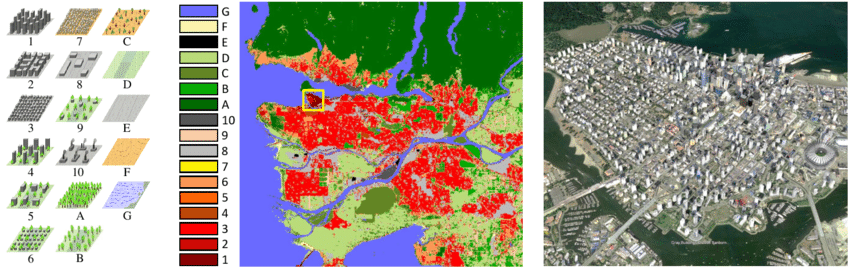
\includegraphics[width=0.9\linewidth]{images/schematic-lcz.png}
  \caption{The LCZ classes as schematics on the left and matching of classes for a city in the centre. Image taken from \cite{zhu_so2sat_2019}.}\label{fig:lcz_classes}
\end{figure*}


\subsection{Distributed Array Computation}
\label{subsec:distributed_array_computation}
General array computation is used in a lof of scientific fields nowadays.
Simulation of atomic levels or measurements of fuel are fine grained enough to have huge data amounts
and they still need to be processed.
One elegant way to solve this is the use of distributed computing. By using multiple machines at once
the computing time should go down while the available memory increases.
But writing distributed programs from scratch is hard problem especially for scientists that have limited amount
of experience with computing in comparison to computer scientists.

\subsection{MPI}
\label{subec:mpi}
\gls{MPI} is a message-passing standard published from the Message-Passing Interface Forum. It is currently available in version 3.1 \cite{message_passing_interface_forum_mpi_nodate}.
\enquote{The goal of the Message-Passing-Interface, simply stated, is to develop a widely used standard for writing message-passing programs}\cite{message_passing_interface_forum_mpi_nodate}.
With this goal \gls{MPI} is today often used in \gls{HPC}, especially in Grid Computing. The standard interface allows to pass results or data between different processes or nodes.
Due to \gls{MPI} being a standard multiple implementations exist, that support different versions of the standard.
% TODO: Add citation
Some of these implementations OpenMPI \cite{noauthor_open_nodate} and Intel MPI \cite{noauthor_intel_nodate}, which are available on our compute ressources.

\subsection{HEAT}
\label{subsec:heat}
\gls{HeAT} is introduced in \cite{krajsek_helmholtz_nodate}. HeAT aims to be a mathemtical library for distributed computations.
It conforms to a Numpy \cite{noauthor_numpy_nodate} interface and make all distributed calculations transparent. To move from executing \gls{HeAT} scripts to executing them parallel
or distributed one just needs to change the execution command to MPI.
This is due to \gls{HeAT} wrapping PyTorch as implementation with the correct \gls{MPI} synchronization to distribute the calculation.

To perform the calculation distributed correctly \gls{HeAT} adds a new data structure: the DNDArray. Users of other libraries
recognize the general interface of Numpy arrays or PyTorch Tensors, but extended by a split parameter.
The split parameter allows to control the axis, which \gls{HeAT} distributed across the different nodes.

Although, the distribution is transparent besides the split parameter, several pitfalls exist.
When reshaping or splicing the dataset one has to potentially rebalance the dataset. Additionally, this could incurr communication effort
to redistribute the dataset across the nodes.
Another pitfalls especially for developers comming from the distributed programming, lies in all processes needing to call all \gls{HeAT} methods.
While in traditional \gls{MPI} one discriminates between the processes based on the rank, in \gls{HeAT} all nodes need to access all functions and DNDArrays or the
programm could lockup.

Lastly, \gls{HeAT} provides the load utility for distributed loading of datasets. Through the usage of all nodes at the same time IO is maximized and the data
is splitted already during loading. Therefore, calculations can start right away without the need to distribute the data.
\cite{krajsek_helmholtz_nodate}


\subsection{Local Climate Zone Classification}
\label{subsec:local_climate_zone_classification}

\gls{LCZ}s are a scheme formally proposed by \citeauthor{stewart_local_2012} in \cite{stewart_local_2012}. The scheme classifies areas based on fabric, land cover, structure
and metabolism into one of 17 \gls{LCZ}s. \cite{xue_applications_2020}
The \gls{LCZ}s are decided by 4 components:
\begin{enumerate}
  \item Height of roughness features
  \item Packing of roughness features
  \item Surface cover around roughness features
  \item Thermal admittance of materials
\end{enumerate}
The different classes can be seen in \cref{fig:lcz_classes}.



\subsection{SO2Sat}
\citeauthor{zhu_so2sat_2019} presented the SO2Sat dataset in \cite{zhu_so2sat_2019}. They describe SO2Sat as a \enquote{valuable benchmark dataset [...], which consists of local climate zone (LCZ) labels of about half a million [...] image patches}.
These images are taken from Sentinel-1 and Sentinel-2. Each image is 32 by 32 pixels and contains 8 channels for Sentinel-1 and 10 channels for Sentinel-2.
After preprocessing these images they were given to domain experts for labelling which follwed a \enquote{carefully designed labelling work flow}.
Through the careful work the dataset achieved a \enquote{overall confidence of 85\%}.
The annotations contains the 17 LCZ classes.
The regions of the dataset are 52 cities.

\subsection{Spectral Clustering}
\label{subsec:spectral_clustering}

\begin{algorithm}[b]
  \SetKwData{Laplace}{\(L\)}\SetKwData{Adj}{\(W\)}
  \KwData{Similariy matrix \(S\), number \(k\) of clusters}
  \KwResult{Clusters \(A_1, \ldots, A_k\) }
  Construct a similarity graph\;
  \Adj \(\leftarrow\) weighted adjacency matrix\;
  \Laplace \(\leftarrow\) computeLaplacian(\Adj)\;
  \(u_1, \ldots, u_k \leftarrow\) computeEigenvectors(L)\;
  \(U\) \(\leftarrow\) Matrix with columns \(u_1, \ldots, u_k\)\;
  \ForEach(){\(i = 1, \ldots, n\)}{
    \(y_i\) \(\leftarrow\) vector corresponding to the \(i\)-th row of \(U\)
  }
\(C_1, \ldots, C_k \leftarrow\) kMeans(\(y_1, \ldots, y_n\))\;

  \caption{Basic Spectral Clustering}\label{alg:basic_spectral}
 \end{algorithm}

\enquote{Spectral Clustering is the process of partitioning data samples into
\(k\) groups based on graph theory} \cite{krajsek_helmholtz_nodate}. Therefore,
to derive the formulation of Spectral Clustering we introduce the undirected graph \(G=(V, E)\).
We consider the graph as weighted by assigning each edge an weight \(w_{ij}\). As the graph
is unidrectional, the weight is identical for \(w_{ij} = w_{ji} \).
% Degree Matrix
We define the degree of a vertex \(v_i \in V\) by iterating over all vertices \(v_j \in V\) that are connected to \(v_i\).
Therefore, the weight of the edge is positive:
\[d_i = \sum_{j=1}^n w_{ij}\]
Using the degree defined before, we define the degree matrix \(D\) as the diagonal matrix whith the degrees \(d_1, \ldots, d_n\) on the diagonal.
\cite{von_luxburg_tutorial_2007}
% Weights Matrix
For 2 subsets of indices \(A, B\) we define the weights matrix \cite{von_luxburg_tutorial_2007}:
\[W(A, B) := \sum_{i \in A, j \in B} w_{ij}\]


There are several possible ways to construct such a similarity graph from two datasets.
The following three are used often for spectral clustering:
\begin{itemize}
  \item Fully connected
  \item Symmetric
  \item \(\epsilon\)-Neighbourhood
\end{itemize}
According to \cite{von_luxburg_tutorial_2007} there is no theoretical work on the choosing of one method over
another.

Using the constructed similarity graph we need to calculate the spectrum of the similarity matrix.
This is done by constructing the Laplacian defined via
\[L = W - D\]
using \(W, D\) as defined earlier.

The Lanczos algorithm \cite{lanczos_iteration_1950} is used to calculate the eigenvalues and eigenvectors from the laplacian.
When using the \(k\) smallest eigenvalues and the korresponding eigenvectors \(e_1, \ldots, e_k\) we can embedd the dataset.

Now a clustering can be performed in the smaller embedding space of the eigenbasis using another algorithm, e.g. KMeans.
The overall algorithm can be found in algorithm \ref{alg:basic_spectral}.

\begin{figure}
  
\includegraphics{images/spectral_example.png}
  \caption{2 Half-Moon example for clustering performance of spectral clustering. Taken from \cite{noauthor_23_2020}.}
  \label{fig:spectral_example}
\end{figure}

One of the most common examples for spectral clustering can be seen in \cref{fig:spectral_example}. Spectral Clustering is able to
separate the both datasets. This is often compared with KMeans which fails to correctly recognize the different clusters when using the euclidean distance.

\subsection{Distance Metrics}
\label{subsec:distance_metrics}
For the spectral clustering the distance between samples needs to be measured. Depending on the data different ways to measure the distance are implemented in \gls{HeAT}.

\subsubsection{Euclidean Distance}
The euclidean distance is a default way to measure the distance. The euclidean distance of two points \(X = (x_1, \ldots, x_n ), X' = (x_1', \ldots, x_n')\) is commonly defined  as:
\[
  d\left(X, X'\right) = \sqrt{{(x_1' - x_1)}^2 + \ldots + {(x_n' - x_n)}^2}
\]
It is fast and easy to calculate, but it allows only for linear separatation with most algorithms.

\subsubsection{Radial Basis Function Kernel}
The RBF kernel is a kernel that wraps the euclidean distance \(d\) \cite{vert_primer_2004}:
\[
  K\left(X, X'\right) = \exp(-\gamma d(X, X'))
\]
The RBF kernel is a measure of similarity and augments the effects of the euclidean distance due to the exponential function.
It allows to seperate non-linear data with many algorithms.


\subsection{Clustering Evaluation Metrics}
\label{subsec:clustering_evaluation_metrics}

Evaluating clusters is more complicated than evaluating classification or other supervised machine learning tasks.
Unsupervised tasks can be evaluating using interal or external metrics. While, internal metrics are derived from the algorithm itself e.g. Cluster purity, external metrics need labels for the dataset.

Due to in this work used dataset having labels, this section is going to focus on external metrics.
For the here presented metrics we define \(C\) as the ground truth classes and \(K\) as the clustering assignment.
ON this basis we define the following:\\
\(a\) - the number of pairs of elements that are in the same set in \(C\) and in the same set in \(K\)\\
\(b\) - the number of pairs of elements that are in different sets in \(C\) and in different sets in \(K\)\\


\subsubsection{Adjusted Rand Index}
The \gls{ARI} measures the similarity of two assignments. While the raw Rand Index has problems with random assignments, the \gls{ARI} assigns a score close to \(0\)
to random assignments.
The raw Rand Index is mathematically given by \cite{noauthor_23_2020} as
\[RI = \frac{a + b}{C_2^{n_{samples}}}\]
When adjusting this index for random assignments we yield:
\[ARI = \frac{RI - \mathbb{E} [RI]}{\max (RI) - \mathbb{E} [RI]}\]


\begin{figure*}
  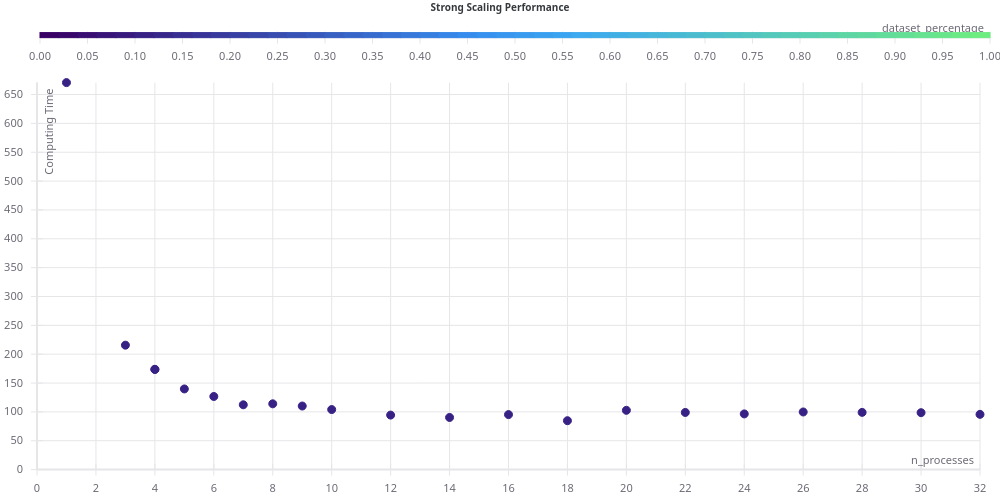
\includegraphics[width=0.9\linewidth]{images/strong_scaling_chart.png}
  \caption{Strong scaling behaviour of the Spectral Clustering algorithm. Baseline of 1 node with \(6489s\) excluded for visual purposes.}\label{fig:strong_scaling}
\end{figure*}





% use section* for acknowledgment
\ifCLASSOPTIONcompsoc
  % The Computer Society usually uses the plural form
  \section*{Acknowledgments}
\else
  % regular IEEE prefers the singular form
  \section*{Acknowledgment}
\fi
The authors would like to thank the Steinbuch Centre for Computing for providing the necessary compute power for
performing the here presented profiling.
Furthermore, we would like to thank the HeAT team for providing support regarding any troubles and questions.


In the bibliography, use \texttt{\textbackslash textsuperscript} for ``st'', ``nd'', \ldots:
E.g., \enquote{The 2\textsuperscript{nd} conference on examples}.
When you use \href{https://www.jabref.org}{JabRef}, you can use the clean up command to achieve that.
See \url{https://help.jabref.org/en/CleanupEntries} for an overview of the cleanup functionality.

% trigger a \newpage just before the given reference
% number - used to balance the columns on the last page
% adjust value as needed - may need to be readjusted if
% the document is modified later
%\IEEEtriggeratref{8}
% The "triggered" command can be changed if desired:
%\IEEEtriggercmd{\enlargethispage{-5in}}

% Enable to reduce spacing between bibitems (source: https://tex.stackexchange.com/a/25774)
% \def\IEEEbibitemsep{0pt plus .5pt}

\bibliographystyle{IEEEtranN} % IEEEtranN is the natbib compatible bst file
% argument is your BibTeX string definitions and bibliography database(s)
\bibliography{paper}

\ \\ % empty line after bibliogpraphy and that statement
All links were followed on 15. February 2021
\end{document}
